\chapter{序論}
\label{chap:introduction}

本章では, はじめに本研究における背景を述べる.ついで, 問題意識を踏まえた上での目的, 製作者の仮説を述べる. 最後に本論文の構成を示す.

\section{背景}
本節では, 本研究の背景としと人と人との繋がりで構成されている現代社会について述べる. ついで人との繋がり形成におけるコミュニケーション上での表情の重要性を述べ, 最後に現代社会における人との関係性を構築する手段が多様化している様子を述べる.

%\begin{quotation}
%\end{quotation} 引用をする際にはこれを使用する

\subsection{人と人との繋がりで構成されている社会}
ヒトは誕生から現代にかけて社会を形成し,その中で集団を作って生活を送ってきた. 社会性をもつ生き物として, 交友関係を広げ, 協力をして日々を生きている. 職場, 学校, 近所, そして家族など人との繋がりは必要不可欠な要素である. 日本人の平均寿命はWHOの調査で84.2歳\cite{WHO_reserch}と言われ,1日1人と出会ったとしても30733人と出会うことになり, 人と関わることなしに生活することは不可能である.
\subsection{コミュニケーションにおける表情の重要性}
人との関係構築をする際にはコミュニケーションが必要不可欠である. コミュニケーションにおいて非言語コミュニケーションがもっとも重要とAlbert Mehrabian\cite{rule_of_Mehrabian}は述べており, 会話中の相手の受け取る情報量は非言語コミュニケーションが93\% を占め, その中でも視覚情報は55\% を占めると言われている. その中でも,人の表情はその人の内面を表しており相手のことを判断するときに重要な判断材料となる.
%表情,笑顔が重要な理由を出す
\begin{figure}[htbp]
    \begin{center}
       \fbox{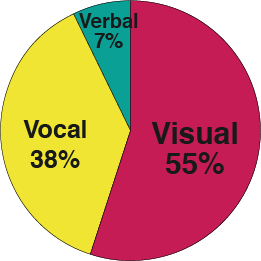
\includegraphics[width=50mm,bb=0 0 261 261]{mehrabian.jpg}}
    \end{center}
    \caption{メラビアンの法則}
    \label{fig:mehrabian}
\end{figure}


\subsection{人との繋がり形成の多様化}
人との繋がりについて書く

\section{本文書の構成}

第1章の最後は、文書全体の構成を大まかに書くとよいらしい。

第\ref{chap:introduction}章では本テンプレートの概要みたいなものを書いた。第\ref{chap:howto}章では、本テンプレートの使い方を説明する。第\ref{chap:latex}章で図表や数式の挿入など代表的な\LaTeX コマンドを解説する。第\ref{chap:conclusion}章では、『序論』で始めたら『結論』で終われと書いた手前書かざるを得ないので、なにか結論らしいことを書く。付録として、テンプレートのサンプルになるように無理矢理ゴミを添付する。
